% 保存为 presentation.tex
\documentclass{beamer} % 必须声明beamer文档类

%---------- 主题设置 ----------
\usetheme{Madrid}      % 内置主题(推荐新手使用)
\usecolortheme{seahorse} % 配色方案
\setbeamertemplate{navigation symbols}{} % 隐藏导航图标

%---------- 中文字体配置 ----------
%\usepackage[UTF8]{ctex}
%\setCJKmainfont{SimHei} % 设置中文字体(确保系统已安装)

%---------- 常用宏包 ----------
\usepackage{graphicx}  % 插入图片
\usepackage{listings}  % 代码高亮
\usepackage{animate}   % 动画支持
\usepackage{tikz}      % 矢量绘图
\usepackage{subcaption}
\usepackage{color}
\usepackage{listings}
\usepackage{xcolor} % 定制颜色
\definecolor{mygreen}{rgb}{0,0.6,0}
\definecolor{mygray}{rgb}{0.5,0.5,0.5}
\definecolor{mymauve}{rgb}{0.58,0,0.82}
\lstset{ 
	language=matlab,
	tabsize=4,
	backgroundcolor=\color{white},
	basicstyle = \tiny\ttfamily,
	rulesepcolor= \color{red!20!green!20!blue!20},
	breaklines = true,
	numbers = left,
	numberstyle = \tiny,
	keywordstyle = \color{blue},
	commentstyle = \color{mygreen},
	stringstyle = \color{mymauve}\ttfamily,
	frame = none,
	showspaces = false,
	columns = fullflexible
}

%======================== 幻灯片内容 ========================
\begin{document}

%---------- 标题页 ----------
\title{Wavelets for image processing}
\author{group member: \\Jingrui Zhang, Jiashun He, Jingyuan Meng, Zishen Jiang, Zian Mo}
\date{\today}
\frame{\titlepage}

\begin{frame}
	\frametitle{Outline}
	\LARGE

	\begin{description}
		\item[section 1]
		\item[section 2] Image compression
	\end{description}
\end{frame}

\begin{frame}
	\frametitle{section 2}
	\centering{\LARGE{\textbf{Image compression}}}
\end{frame}

\begin{frame}
	\frametitle{Image compression}
	\begin{figure}
		\centering
		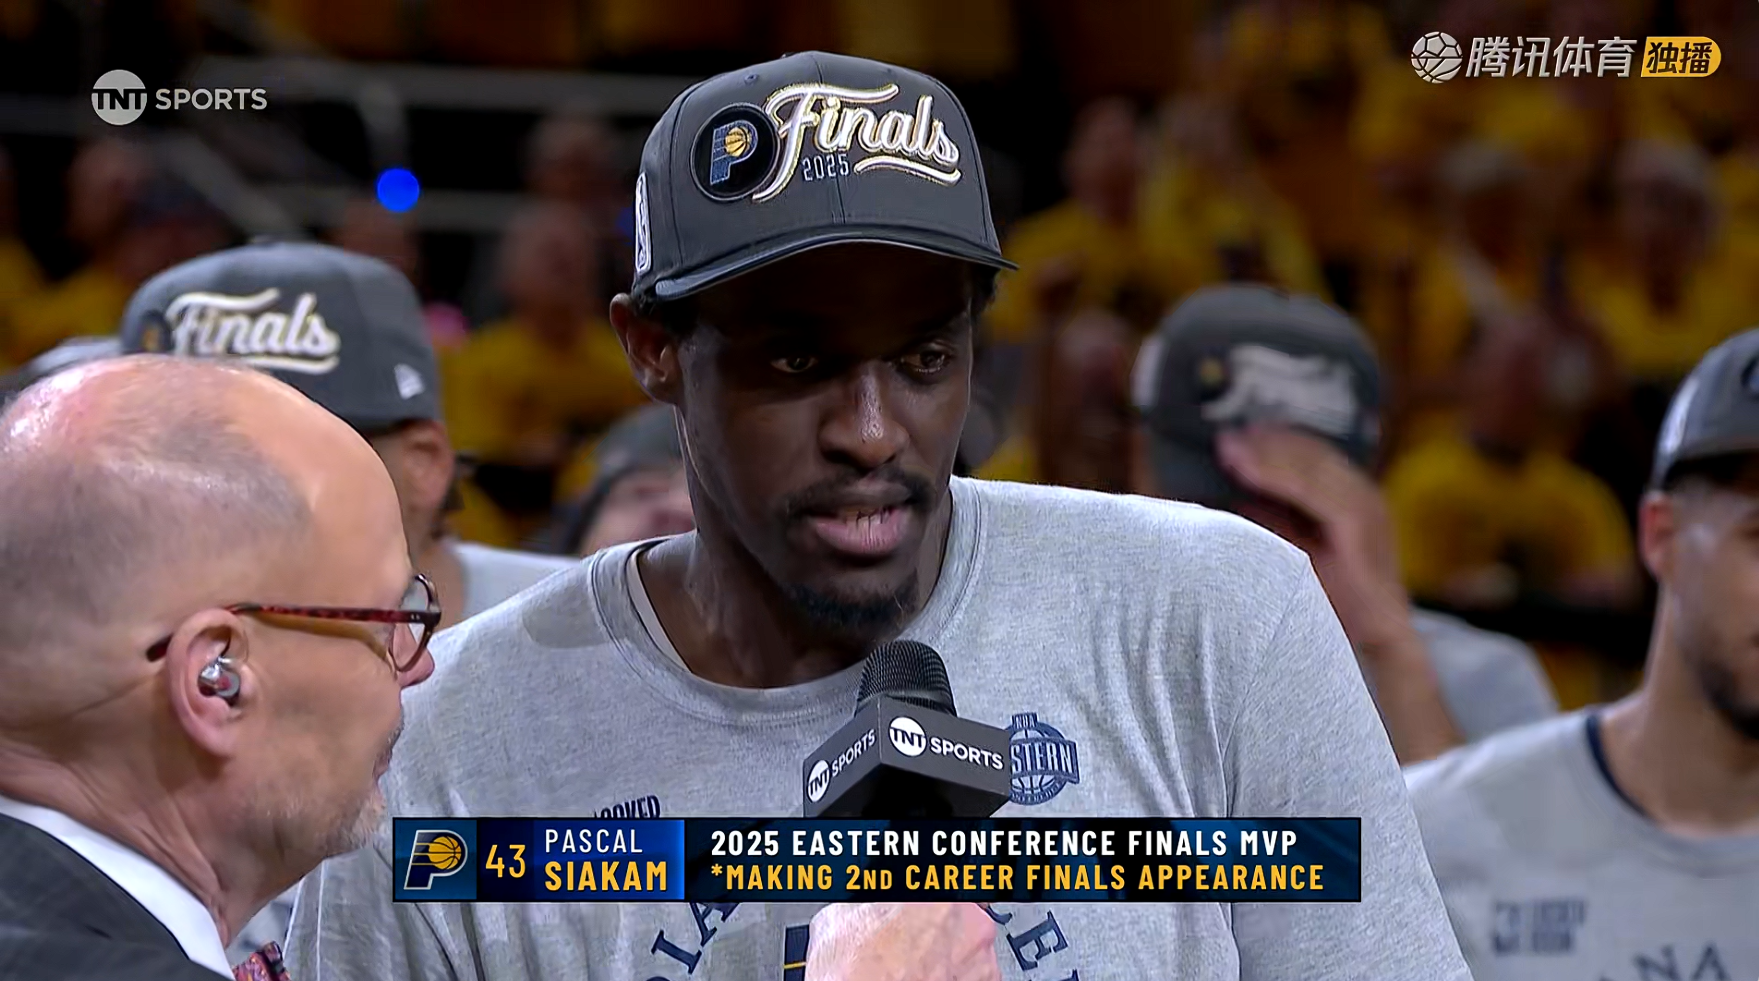
\includegraphics[width=0.8\textwidth]{fig/Siakam.png} % 替换为你的图片路径
		\caption{Siakam won 2025 NBA eastern conference finals MVP}
		\label{fig:Siakam}
	\end{figure}
\end{frame}

\begin{frame}
	\frametitle{Image compression}
	The picture is stored as RGB array in computer.
	\begin{figure}
		\centering
		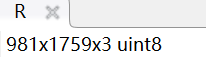
\includegraphics[width=0.45\textwidth]{fig/pic_Siakam_RGB_size.png} % 替换为你的图片路径
		\caption{Using MATLAB function "imread" to get its corresponding RGB array}
		\label{fig:Siakam_size}
	\end{figure}
	{\color{red}The corresponding RGB array is quite Huge!}
\end{frame}

\begin{frame}
	\frametitle{Image compression}
	{\color{blue}Our Purpose: Compress the image to reduce storage space}\\
	For convenience, we convert the color image into a grayscale image.
	\begin{figure}
		\centering
		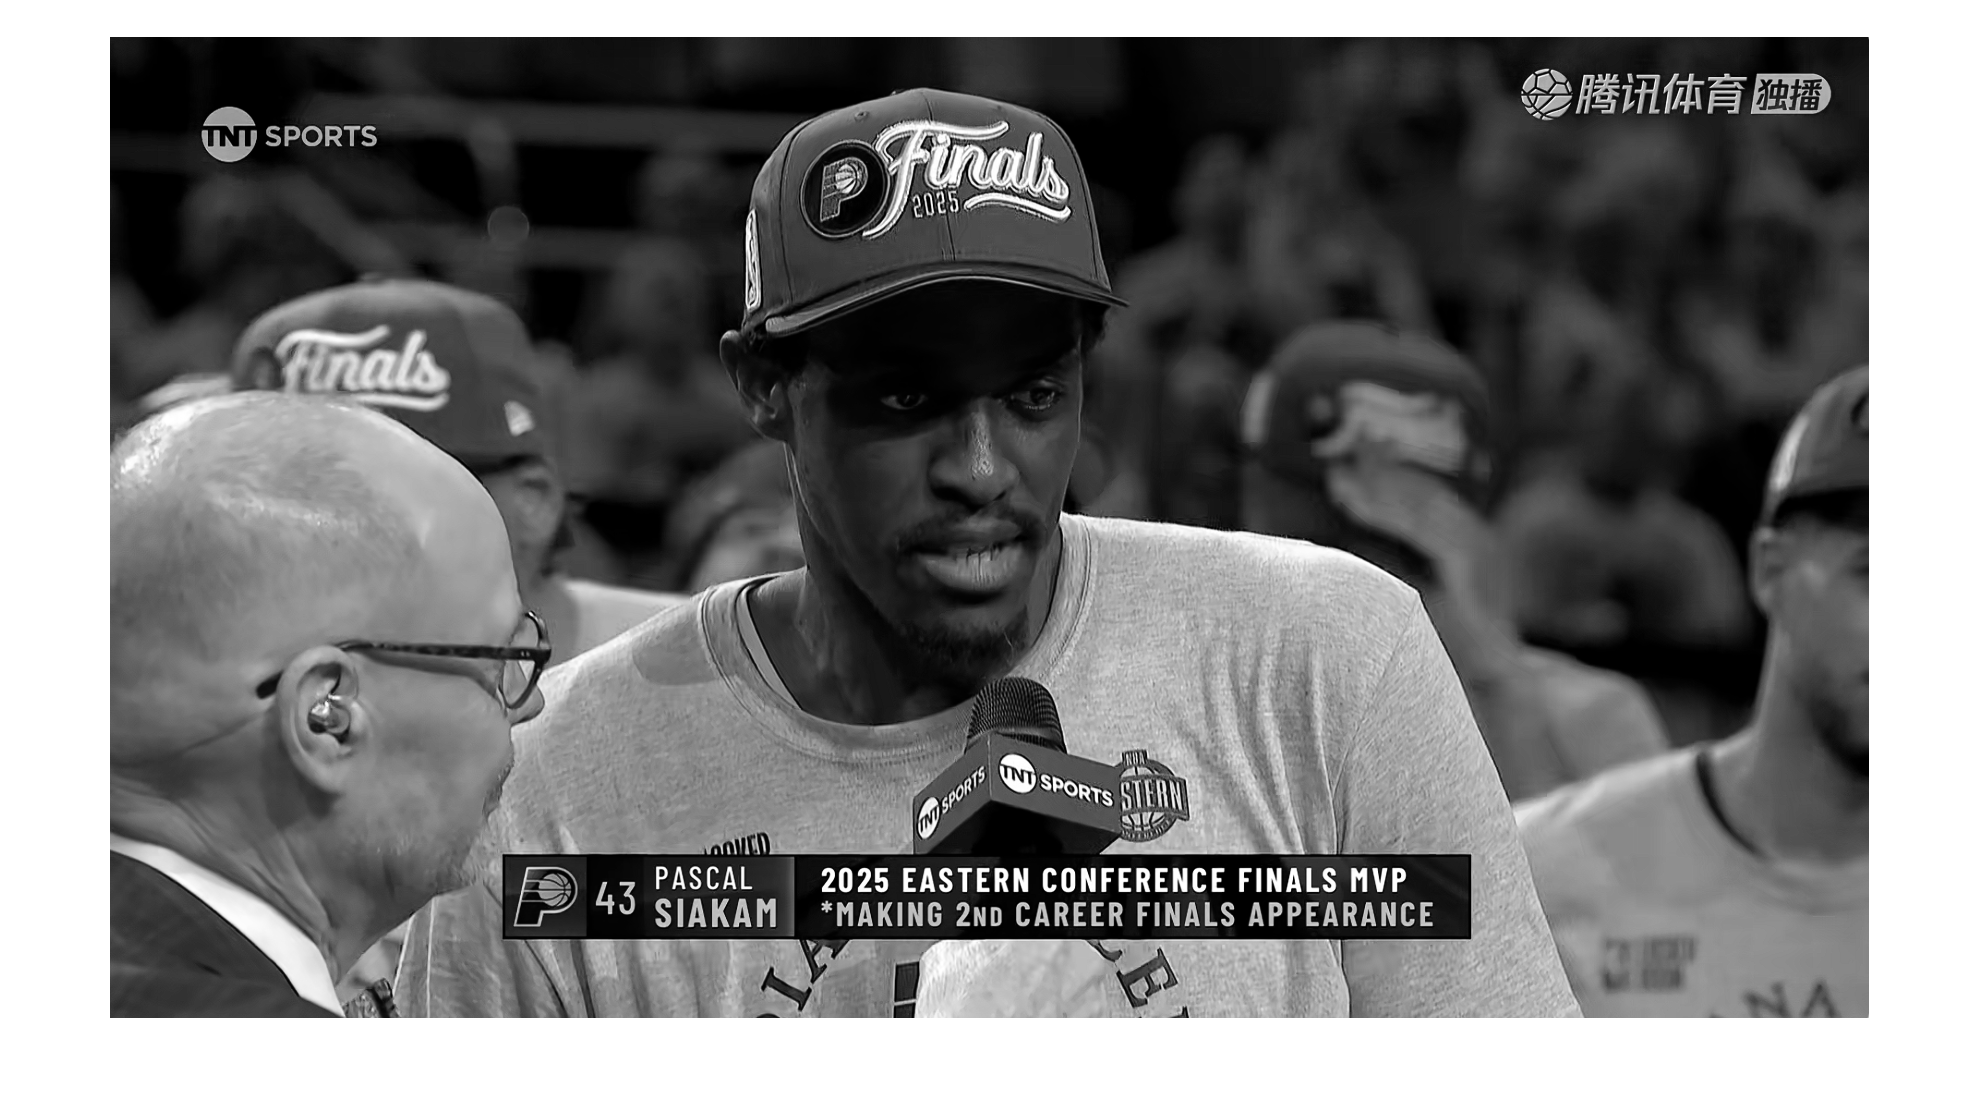
\includegraphics[width=0.8\textwidth]{fig/Siakam_gray.png} % 替换为你的图片路径
		\caption{Using MATLAB function "rgb2gray" to convert the image}
		\label{fig:Siakam_gray}
	\end{figure}
\end{frame}

\begin{frame}
	\frametitle{Image compression}
	The RGB array can be viewed as a combination of three matrices, \\
	while a grayscale image is only decided by a Grayscale matrix.
	$$\Downarrow\Downarrow\Downarrow\Downarrow$$
	We can compress a color image \\
	\textbf{as long as we can compress a grayscale image}.
\end{frame}

\begin{frame}
	\frametitle{Image compression}
	The RGB array can be viewed as a combination of three matrices, \\
	while a grayscale image is only decided by a Grayscale matrix.
	$$\Downarrow\Downarrow\Downarrow\Downarrow$$
	We can compress a color image \\
	\textbf{as long as we can compress a grayscale image}.
	\\ \ \\\ \\
	\centering{\LARGE \color{blue}Then, how to do that?}
\end{frame}

\begin{frame}
	\frametitle{Image compression}
	\begin{block}{Theorem 2.1}
		Let $\{u_{i}\}_{i=1}^{m}$ is a set of \textbf{orthonormal bases} of $\mathbb{R}^{m}$, $\{v_{i}\}_{i=1}^{n}$ is a set of \textbf{orthonormal bases} of $\mathbb{R}^{n}$, then
		$$\{u_{i}\times v_{j}\ |\ i = 1,\cdots m, j=1,\cdots n\}$$
		is a set of \textbf{orthonormal bases} of $\mathbb{R}^{m\times n}$.
	\end{block}
	Meanwhile, for an an integer $num$, if
	\begin{equation}
		\exists\ q \in\mathbb{N}_{+},\ num = 2^{q}, \tag{2.1}\label{20250802imagecompression1}
	\end{equation}
	we can get a set of orthonormal bases of $\mathbb{R}^{num}$ using following matlab code.
\end{frame}
\begin{frame}[fragile]
	\frametitle{Image compression}
	\begin{block}{Get a set of orthonormal bases of $\mathbb{R}^{num}$(matlab)}
		\begin{lstlisting}
			function AnsM = basevecM_D(num) % Unitization
				AnsM = orthvecM_D(num);
				len = size(AnsM, 1);
				for i = 1:len
					AnsM(i,:) = AnsM(i,:)./sqrt(AnsM(i,:)*(AnsM(i,:)'));
				end
			end
			
			function AnsM = orthvecM_D(num) % Get an orthogonal basis
				AnsM = orthvecM_D1(num);
				AnsM = [ones(1, num); AnsM];
			end
			
			function AnsM = orthvecM_D1(num) 
			
			if num == 2
				AnsM = [1, -1];
			else 
				tempM1 = orthvecM_D1(num/2);
				tempM2 = zeros(size(tempM1, 1), num/2);
				tempM3 = ones(1, num/2);
				AnsM = [tempM3, -tempM3; tempM1, tempM2; tempM2, tempM1];
			end
			end
			
		\end{lstlisting}
	\end{block}
\end{frame}
\begin{frame}
	\frametitle{Image compression}
	Then if both $m$ and $n$ satisty the condition \eqref{20250802imagecompression1}, we can get  sets of \textbf{orthonormal bases} of $\mathbb{R}^{m}$ and $\mathbb{R}^{n}$  respectively. ($\{u_{i}\},\{v_{j}\}$)\\ \ \\
	Therefore, $\forall\ A \in \mathbb{R}^{m\times n},\ \exists\ \omega_{i,j}\in\mathbb{R}, i = 1, \cdots m, j = 1, \cdots, n$
	\begin{equation}
		A = \sum_{i,j}\omega_{i,j}\ \cdot \ u_{i} \cdot v_{j}^{T}. \tag{2.2}\label{20250802imagecompression2}
	\end{equation}
	Let $W = (\omega_{i,j})$. We can covert $W$ to $A$ by \eqref{20250802imagecompression2}, which means we only need to store W.
\end{frame}
\begin{frame}
	\frametitle{Image compression}
	{\color{blue}How can we get W?}\\ \ \\
	As $\{u_{i}\},\{v_{j}\}$ are sets of \textbf{orthonormal bases} of $\mathbb{R}^{m}$ and $\mathbb{R}^{n}$,
	$$u_{a}^{T}Av_{b} = \sum_{i,j}\omega_{i,j}\ \cdot \ (u_{a}^{T}u_{i}) \cdot (v_{j}^{T}v_{b}) = \omega_{a,b}.$$
	Let $M = (u_{1},u_{2},\cdots,u_{m}),\ N = (v_{1},v_{2},\cdots,v_{n}).$ Then
	$$M^{T}AN=W.$$
	Meanwhile, since M, N are \textbf{orthogonal matrices},
	$$MWN^{T}=(MM^{T})\cdot A\cdot(N^{T}N) = A.$$
\end{frame}
\begin{frame}
	\frametitle{Image compression}
	{\color{red}How can we compress the image?}\\ \ \\
	Formula \eqref{20250802imagecompression2} indicates the basis linear representation of $A$:
	$$A = \sum_{i,j}\omega_{i,j}\ \cdot \ u_{i} \cdot v_{j}^{T}.$$
	The coefficient $\omega_{i,j}$ reflects \textbf{the influence of  corresponding basis} $u_{i} \cdot v_{j}^{T}$ on the final result $A$.
\end{frame}
\begin{frame}
	\frametitle{Image compression}
	{\color{blue}This means if $\omega_{i,j}$ is too small, the influence of  corresponding basis can be ignored.} Then
	\begin{align*}
		\widetilde{A} = \sum_{i,j}\widetilde{\omega_{i,j}}\ \cdot \ u_{i} \cdot v_{j}^{T},\ \widetilde{\omega_{i,j}} = \left\{
		\begin{aligned}
			 & \omega_{i,j}, & \ |\omega_{i,j}| > \lambda    \\
			 & 0,            & \ |\omega_{i,j}| \leq \lambda
		\end{aligned}
		\right..
	\end{align*}
	$\widetilde{A}$ is an approximation of $A$, while $\lambda$ is image compression strength.\\ \ \\
	Let $\widetilde{W} = (\widetilde{\omega_{i,j}}).$ As long as $\lambda$ is large enough, we can transform $\widetilde{W}$ into a \textbf{sparse matrix} which needs less storage space.\\ \ \\
	Meanwhile, we only need to save $\widetilde{W}$ to store $\widetilde{A}$.
\end{frame}
\begin{frame}
	\frametitle{Image compression}
	{\LARGE Main Process}\\ \ \\
	\begin{enumerate}
		\item Get basis matrixs of $\mathbb{R}^{m}\ and\ \mathbb{R}^{n}$. (M,N)
		\item Use $M^{T}AN=W$ to get coefficient matrix $W$.
		\item Compress matrix $W$ to sparse matrix $\widetilde{W}$.
	\end{enumerate}
	However, the method to get basis matrixs can be used \textbf{only if} m,n satisfy the condition \eqref{20250802imagecompression1}. Commonly, this is not true. We usually \textbf{expand} the original image so that the final expanded image meets this condition and the expanded part is all white.\\\ \\
	{\color{blue}Then we set $\lambda$ equal to $0.5$ and see the result.}
\end{frame}
\begin{frame}
	\frametitle{Image compression}
	\begin{figure}[ht]
		\centering
		\begin{subfigure}[b]{0.45\textwidth}
			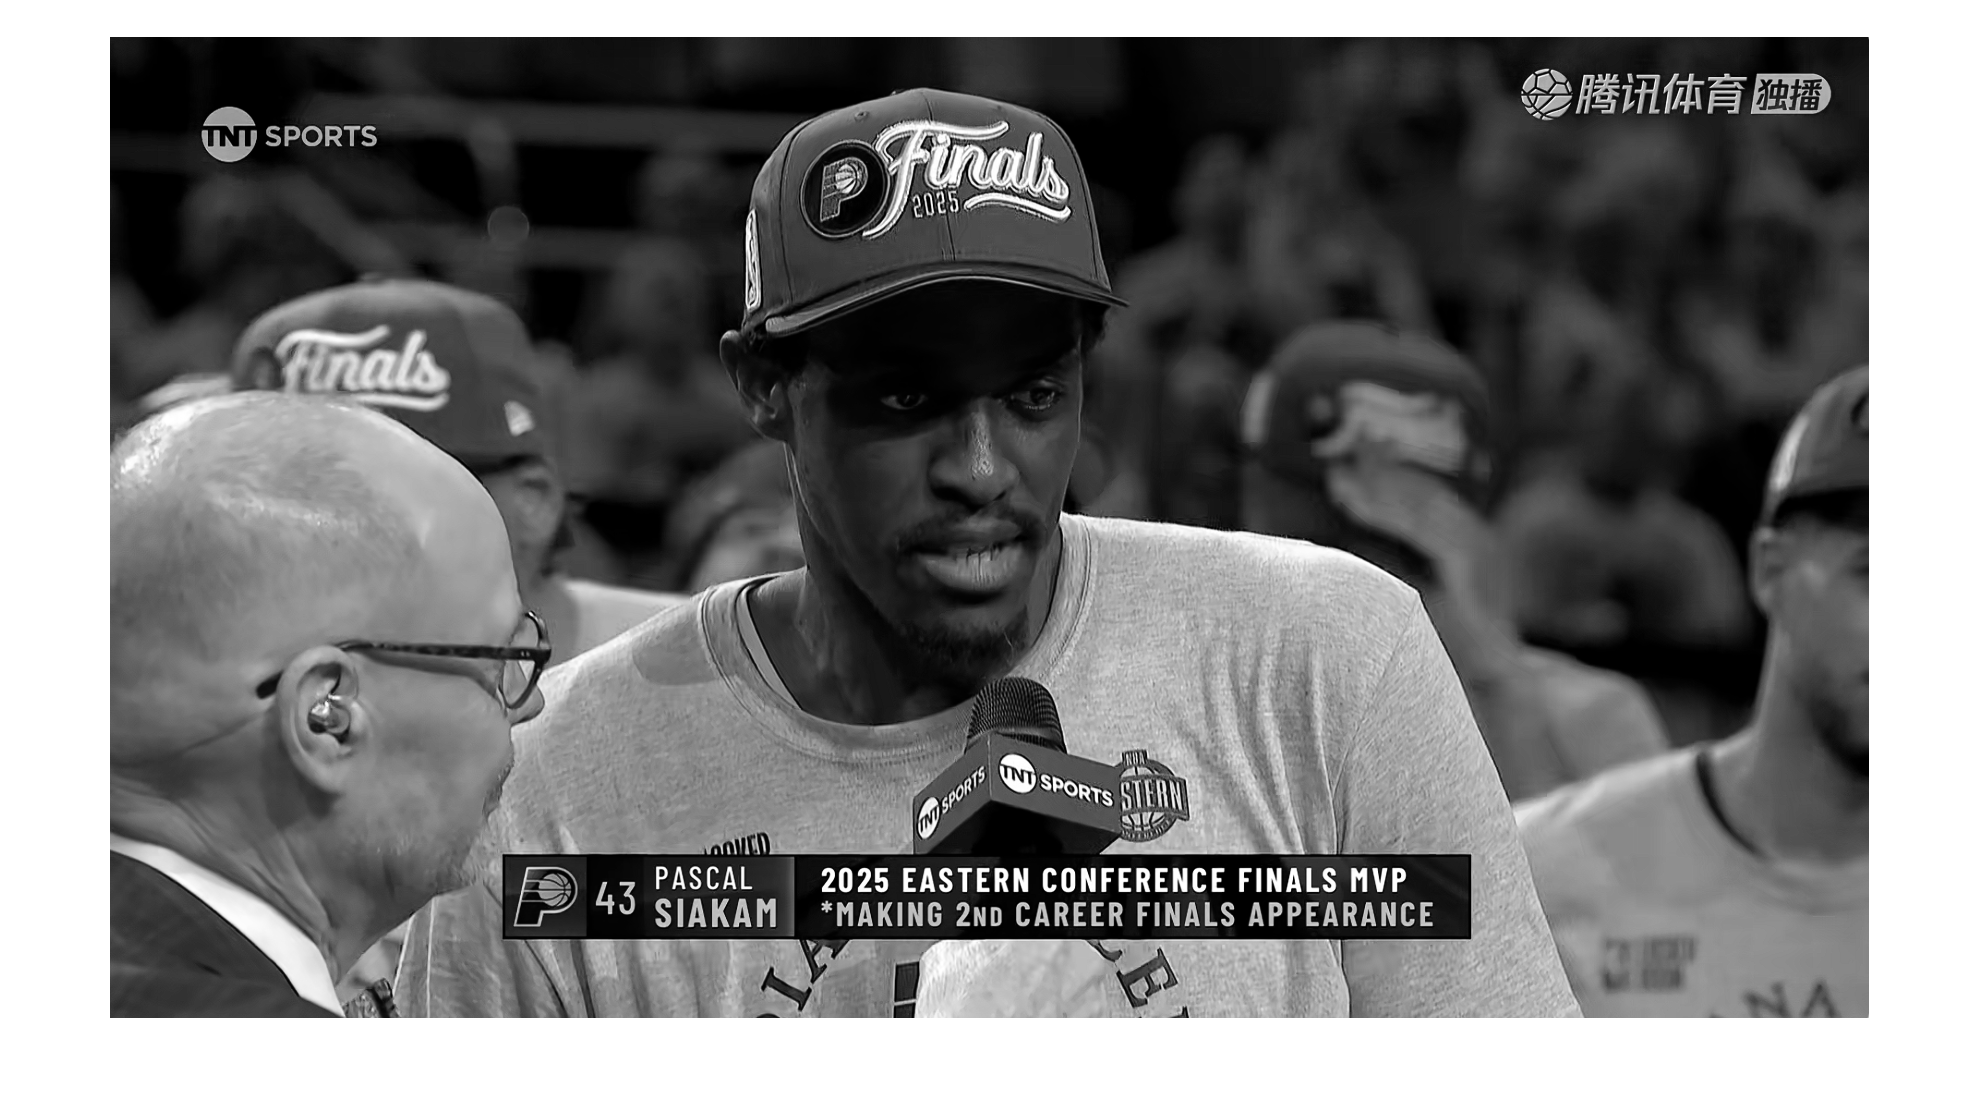
\includegraphics[width=\textwidth]{fig/Siakam_gray.png}
			\caption{Original image}
			\label{fig:20250803Siakam}
		\end{subfigure}
		\hfill % 水平填充,确保两个子图并排
		\begin{subfigure}[b]{0.45\textwidth}
			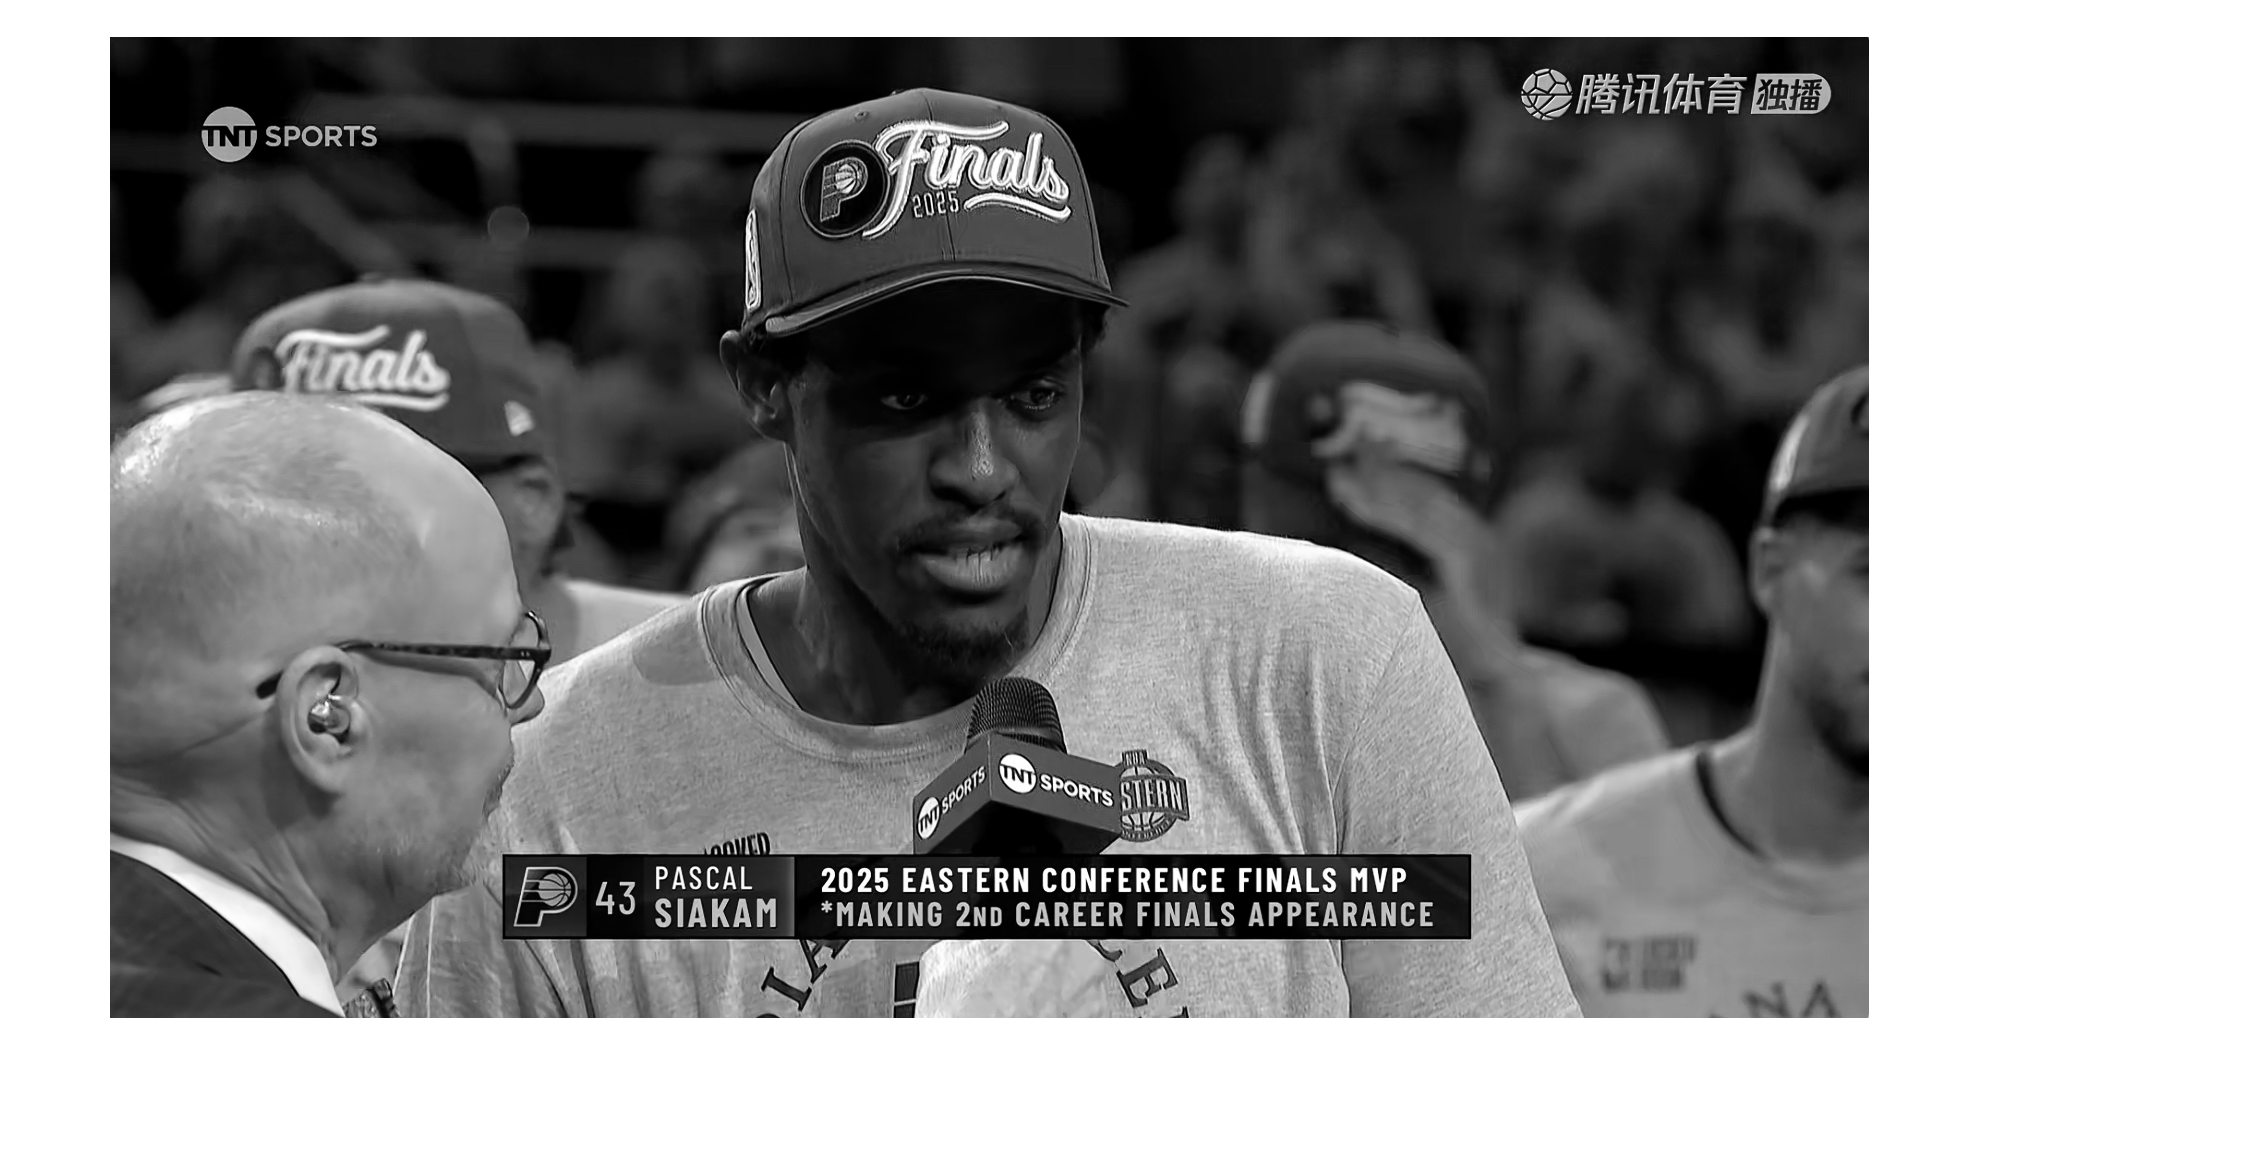
\includegraphics[width=\textwidth]{fig/Siakam_expanded.png}
			\caption{Expanded image}
			\label{fig:20250803Siakam_expanded}
		\end{subfigure}
		\begin{subfigure}[b]{0.45\textwidth}
			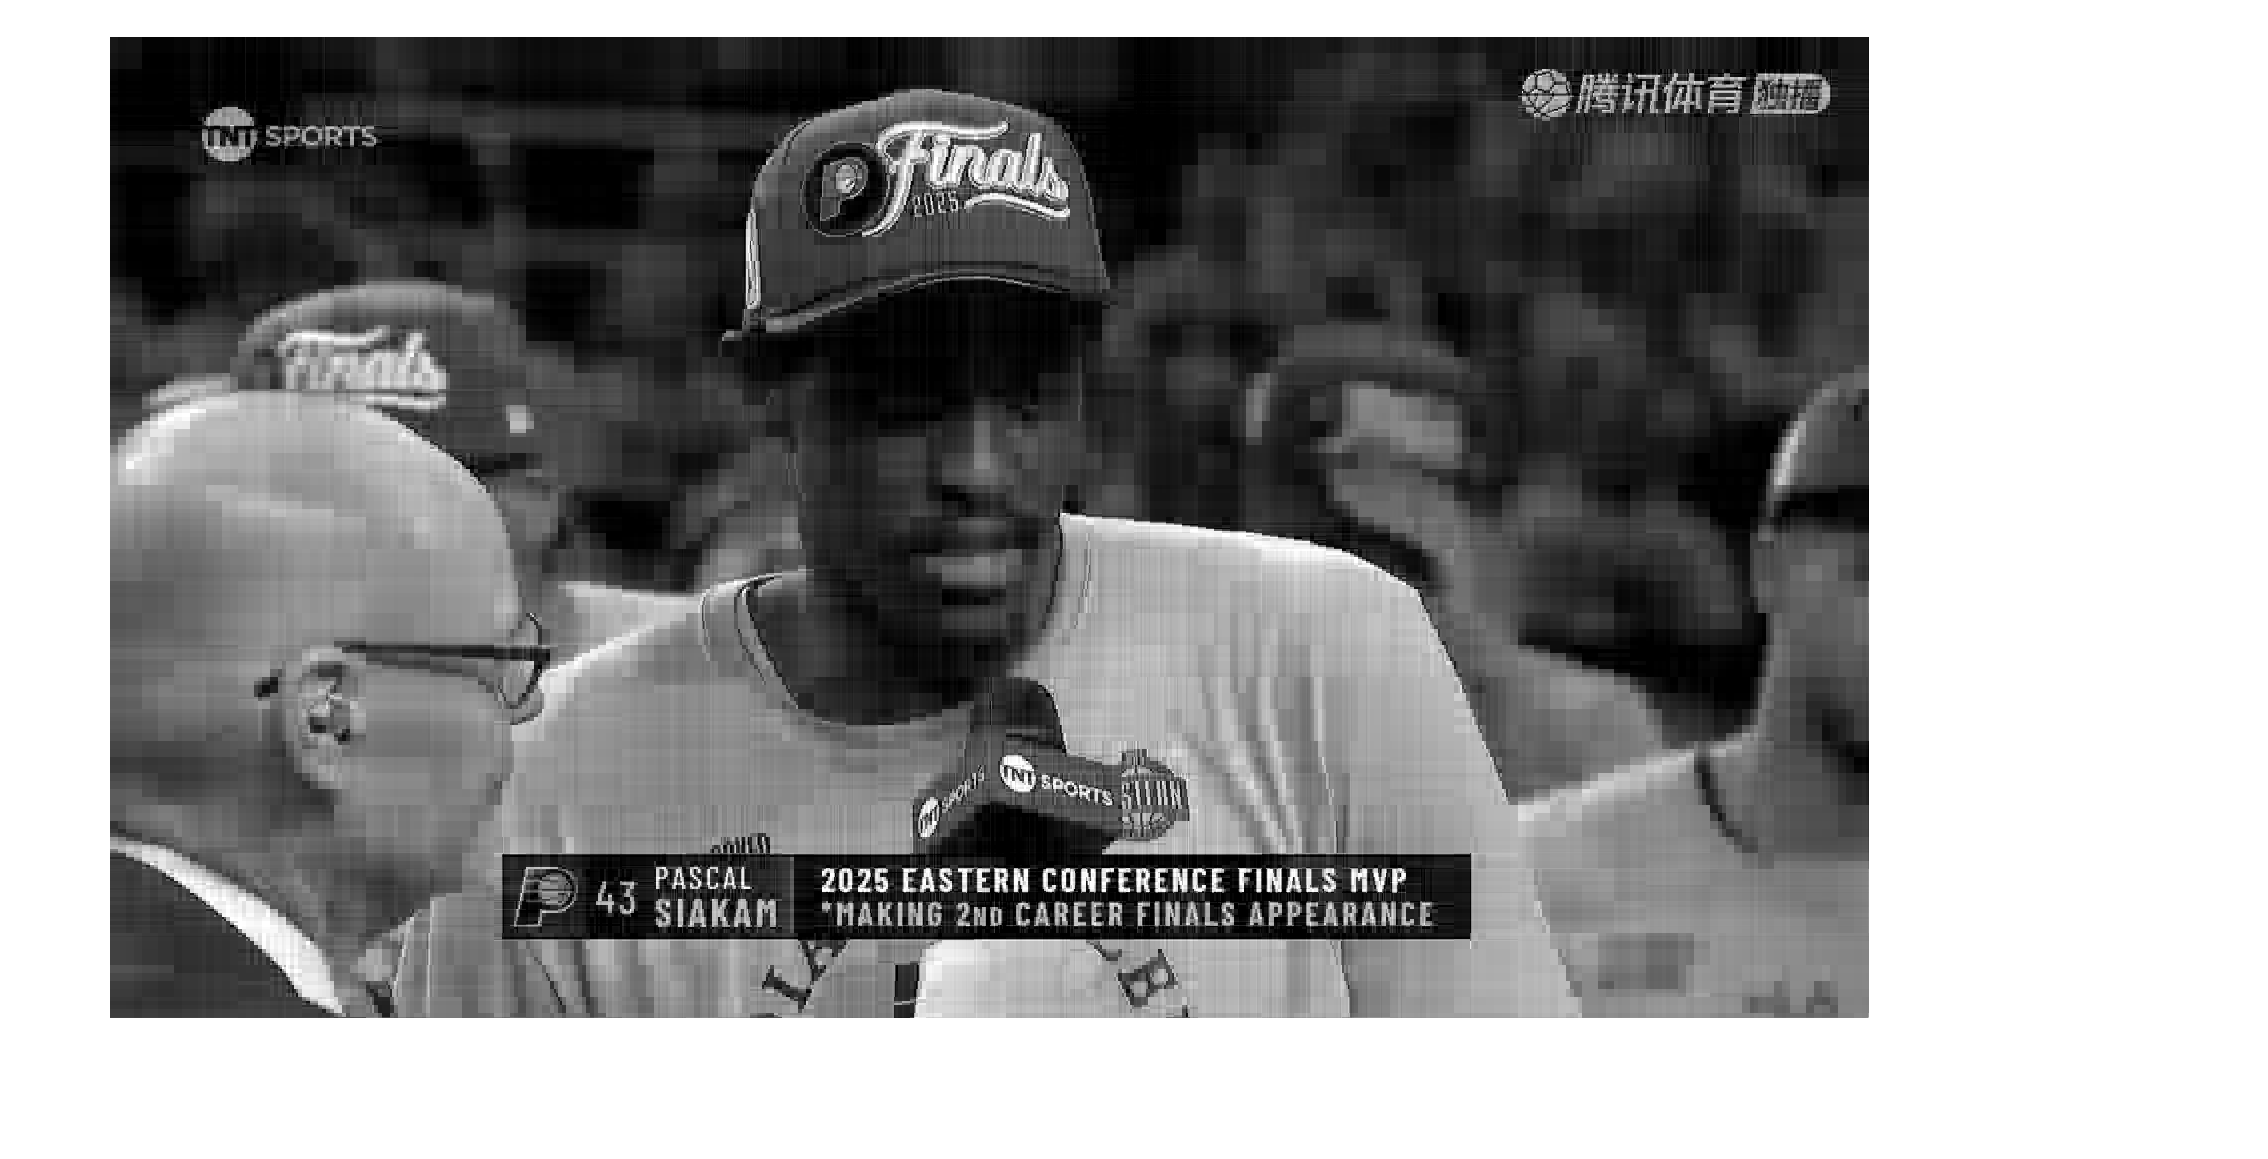
\includegraphics[width=\textwidth]{fig/Siakam_expanded_compressed.png}
			\caption{Compressed expanded image}
			\label{fig:20250803Siakam_expanded_compressed}
		\end{subfigure}
		\hfill % 水平填充,确保两个子图并排
		\begin{subfigure}[b]{0.45\textwidth}
			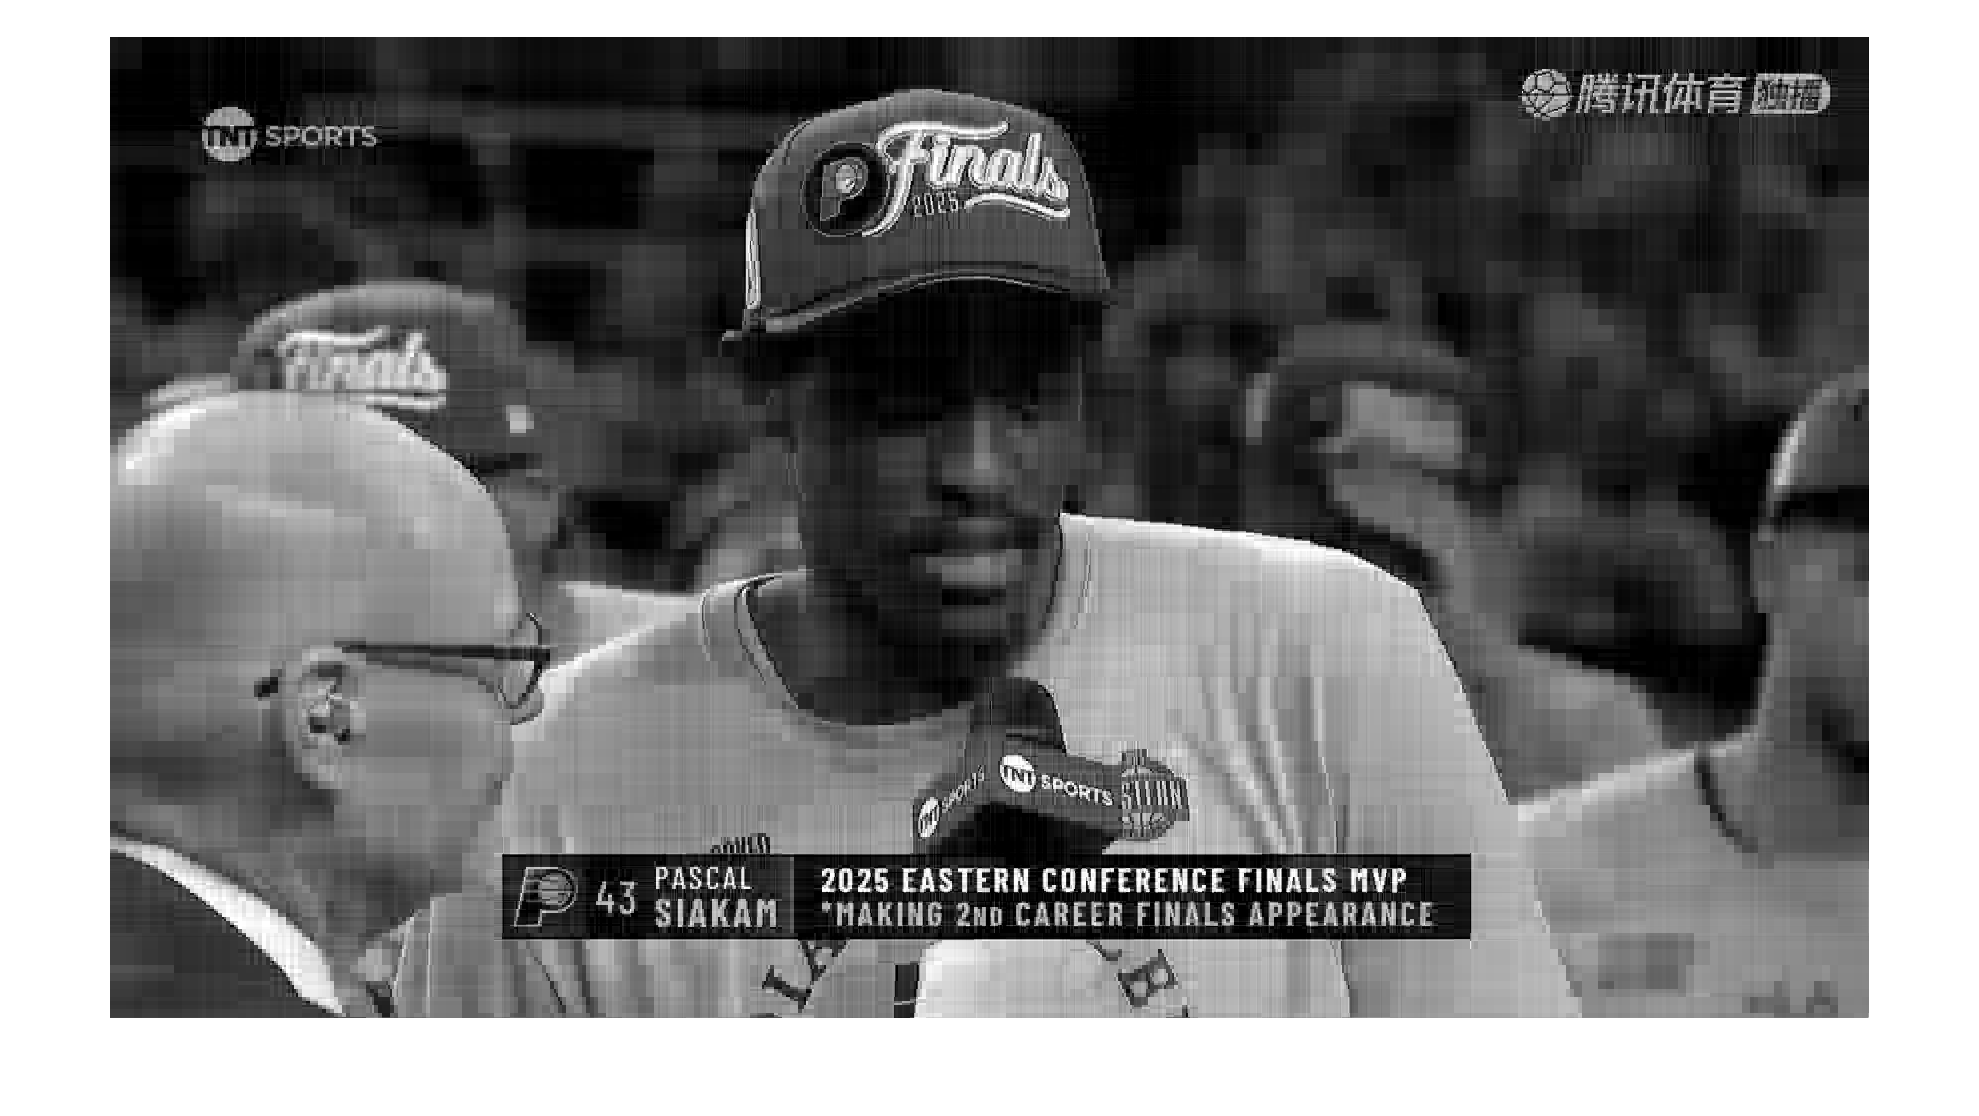
\includegraphics[width=\textwidth]{fig/Siakam_compressed.png}
			\caption{Final image}
			\label{fig:20250803Siakam_compressed}
		\end{subfigure}
		\label{fig:20250803process_total}
	\end{figure}
\end{frame}
\begin{frame}
	\frametitle{Image compression}
	For original image , the size of stored information is $981\times1759 = 1725579$. \\\ \\
	{\color{red} However, after compression, the size of stored information is  only $15364\times2 = 30728$.} \\\ \\
	Indeed, we reduce storage space by compression. However, we also lose much detailed information of original picture. That's why we should change $\lambda$ for different purposes to reach the balance.
\end{frame}
\end{document}